\documentclass{article}
\usepackage{tikz, comment}
\usepackage{pifont}
\usepackage{fontspec}
\usetikzlibrary{arrows, decorations.markings, decorations.pathreplacing}
\begin{comment}
:Title: Not defined yet
:Tags: symmetry;substitution;simplify;reflection;order;number;figure
:Author: Prof.Hu Ji-shan, HKUST
:Slug: No name yet

Description Here.........
\end{comment}
\begin{document}\centering

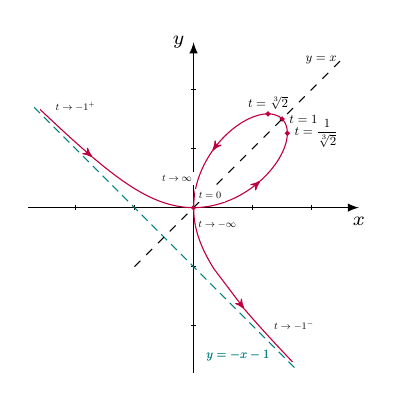
\begin{tikzpicture}[>=latex,xscale=.5*1.5, yscale=.5*1.5][font=\sf\small]

%\draw[xstep=1cm,ystep=1cm,color=gray!80] (0, -1) grid (8, 8);


%\draw[purple, samples=100, smooth, domain=-0.5:0, variable=\t]
% plot ({2*(\t)/(1+(\t)^3)}, {2*(\t)^2/(1+(\t)^3)})--(0,0);


\draw[purple, fill= purple, xscale=1/1.5, yscale=1/1.5] ({0*1.5}, {0*1.5}) circle(0.05);

\draw[purple, fill= purple, xscale=1/1.5, yscale=1/1.5] ({(3/2)*1.5}, {(3/2)*1.5}) circle(0.05)node[black, right, xshift=1, scale=0.5] {$t = 1$};

\draw[purple, fill= purple, xscale=1/1.5, yscale=1/1.5] ({3*(2^(1/3))/(1+2)*1.5}, {3*(2^(1/3))^2/(1+2)*1.5}) circle(0.05) node[black, above, scale=0.5] {$t = \sqrt[3]{2}$};
\draw[purple, fill= purple, xscale=1/1.5, yscale=1/1.5] ({3*(1/2^(1/3))/(1+1/2)*1.5}, {3*(1/2^(1/3))^2/(1+1/2)*1.5}) circle(0.05)node[black, right, xshift=1, scale=0.5] {$\displaystyle t = \frac{1}{\sqrt[3]{2}}$};

\draw[->] (-2.8, 0) -- (2.8, 0)node[below] {\scriptsize$x$} ;
\draw[->] (0, -2.8) -- (0, 2.8)node[left] {\scriptsize$y$} ;

\foreach \x in {-2,-1,1,2}
\draw (\x,2pt/1.5) -- (\x,-2pt/1.5)
node[anchor=north] {}%{\tiny$\x$}
;

\foreach \x in {}
\draw (\x,2pt*2) -- (\x,-2pt*2)
node[anchor=south] {\tiny$\x$}
;
\foreach \y in {-2,-1,1,2}
\draw (-2pt/1.5,\y) -- (2pt/1.5,\y)
node[anchor=east] {}%{\tiny $\y$}
;

\clip[] (-2.7, -2.7) rectangle (2.7, 2.7);

\draw[densely dashed, teal, samples=100, smooth, domain=-2.7:2.7, variable=\x]
plot ({\x}, {-\x-1});
\node[teal, scale=0.5] at (0.75, -2.5) {$y=-x-1$};

\draw[dashed, samples=100, smooth, domain=-1:2.5, variable=\x]
plot ({\x}, {\x}) node[left, scale=0.5] {$y=x$};
\node[teal, scale=0.5] at (0.75, -2.5) {$y=-x-1$};

\clip[] (-2.6, -2.6) rectangle (2.6, 2.6);

\draw[->, >=stealth', purple, samples=150, smooth, domain=-0.9:-0.5, variable=\t]
plot ({3*(\t)/(1+(\t)^3)}, {3*(\t)^2/(1+(\t)^3)})--({3*(-0.5)/(1+(-0.5)^3)}, {3*(-0.5)^2/(1+(-0.5)^3)});

\draw[->, >=stealth', purple, samples=150, smooth, domain=-0.5:0.4, variable=\t]
plot ({3*(\t)/(1+(\t)^3)}, {3*(\t)^2/(1+(\t)^3)})--({3*(0.4)/(1+(0.4)^3)}, {3*(0.4)^2/(1+(0.4)^3)});

\draw[->, >=stealth', purple, samples=150, smooth, domain=0.4:3, variable=\t]
plot ({3*(\t)/(1+(\t)^3)}, {3*(\t)^2/(1+(\t)^3)})--({3*(3)/(1+(3)^3)}, {3*(3)^2/(1+(3)^3)});

\draw[purple, samples=150, smooth, domain=3:20, variable=\t]
plot ({3*(\t)/(1+(\t)^3)}, {3*(\t)^2/(1+(\t)^3)})--(0,0);

\draw[purple, samples=150, smooth, domain=-10:-20, variable=\t]
plot ({3*(\t)/(1+(\t)^3)}, {3*(\t)^2/(1+(\t)^3)})--(0,0);

\draw[->, >=stealth', purple, samples=150, smooth, domain=-10:-3, variable=\t]
plot ({3*(\t)/(1+(\t)^3)}, {3*(\t)^2/(1+(\t)^3)})--({3*(-2)/(1+(-2)^3)}, {3*(-2)^2/(1+(-2)^3)});

\draw[purple, samples=150, smooth, domain=-2:-1.1, variable=\t]
plot ({3*(\t)/(1+(\t)^3)}, {3*(\t)^2/(1+(\t)^3)});


\node[fill=white, scale=0.4] at (0.28,0.21) {$t=0$};

\node[scale=0.4] at (1.7, -2) {$t \to -1^-$};
\node[scale=0.4] at (-2, 1.7) {$t \to -1^+$};

\node[fill=white, scale=0.4] at (-0.28, 0.5) {$t \to \infty$};
\node[scale=0.4] at (0.4, -0.3) {$t \to -\infty$};

%\node[fill=white] at (-0.2/1.2, -0.2/1.2) {\tiny$0$};

\end{tikzpicture}
\end{document}